\documentclass[11pt]{scrartcl}
\usepackage[T1]{fontenc}
\usepackage[a4paper, left=3cm, right=2cm, top=2cm, bottom=2cm]{geometry}
\usepackage[activate]{pdfcprot}
\usepackage[ngerman]{babel}
\usepackage[parfill]{parskip}
\usepackage[utf8]{inputenc}
\usepackage{kurier}
\usepackage{amsmath}
\usepackage{amssymb}
\usepackage{xcolor}
\usepackage{epstopdf}
\usepackage{txfonts}
\usepackage{fancyhdr}
\usepackage{graphicx}
\usepackage{prettyref}
\usepackage{hyperref}
\usepackage{eurosym}
\usepackage{setspace}
\usepackage{units}
\usepackage{eso-pic,graphicx}
\usepackage{icomma}
\usepackage{pdfpages}

\definecolor{darkblue}{rgb}{0,0,.5}
\hypersetup{pdftex=true, colorlinks=true, breaklinks=false, linkcolor=black, menucolor=black, pagecolor=black, urlcolor=darkblue}



\setlength{\columnsep}{2cm}


\newcommand{\arcsinh}{\mathrm{arcsinh}}
\newcommand{\asinh}{\mathrm{arcsinh}}
\newcommand{\ergebnis}{\textcolor{red}{\mathrm{Ergebnis}}}
\newcommand{\fehlt}{\textcolor{red}{Hier fehlen noch Inhalte.}}
\newcommand{\betanotice}{\textcolor{red}{Diese Aufgaben sind noch nicht in der Übung kontrolliert worden. Es sind lediglich meine Überlegungen und Lösungsansätze zu den Aufgaben. Es können Fehler enthalten sein!!! Das Dokument wird fortwährend aktualisiert und erst wenn das \textcolor{black}{beta} aus dem Dateinamen verschwindet ist es endgültig.}}
\newcommand{\half}{\frac{1}{2}}
\renewcommand{\d}{\, \mathrm d}
\newcommand{\punkte}{\textcolor{white}{xxxxx}}
\newcommand{\p}{\, \partial}
\newcommand{\dd}[1]{\item[#1] \hfill \\}

\renewcommand{\familydefault}{\sfdefault}
\renewcommand\thesection{}
\renewcommand\thesubsection{}
\renewcommand\thesubsubsection{}


\newcommand{\themodul}{Halbleiter und Nanotechnologie}
\newcommand{\thetutor}{Prof. Förster}
\newcommand{\theuebung}{Übung 3}

\pagestyle{fancy}
\fancyhead[L]{\footnotesize{C. Hansen}}
\chead{\thepage}
\rhead{}
\lfoot{}
\cfoot{}
\rfoot{}

\title{\themodul{}, \theuebung{}, \thetutor}


\author{Christoph Hansen \\ {\small \href{mailto:chris@university-material.de}{chris@university-material.de}} }

\date{}


\begin{document}

\maketitle

Dieser Text ist unter dieser \href{http://creativecommons.org/licenses/by-nc-sa/4.0/}{Creative Commons} Lizenz veröffentlicht.

\textcolor{red}{Ich erhebe keinen Anspruch auf Vollständigkeit oder Richtigkeit. Falls ihr Fehler findet oder etwas fehlt, dann meldet euch bitte über den Emailkontakt.}

\tableofcontents


\newpage



\section{Aufgabe 1}

\subsection*{a)}

Der Strom aus dem Behälter ist:

\begin{align*}
j_N &= \frac{N}{V} \cdot \frac{<v>}{4} = \frac{\p N}{\p t} \cdot \frac{1}{A} \\
\Leftrightarrow N(t + \d t) &= N(t) - j_{N(t)} \cdot A \cdot \d t \\
\Leftrightarrow n(t + \d t) &= n(t) - \frac{j_{N(t)} \cdot A \cdot \d t}{V} \\
\Leftrightarrow \frac{n(t + \d t) - n(t)}{\d t} &= - \frac{j_{N(t) \cdot A}}{V} = \frac{-n(t) \cdot <v> \cdot A}{V \cdot 4} \\
\underset{\d t \rightarrow 0}{lim} \qquad \frac{\dot{n}}{n} &= \frac{<v> \cdot A}{4V} := \frac{1}{\tau} \\
\hfill \\
\Rightarrow n(t) &= n_0 \cdot e^{-\frac{t}{\tau}}
\intertext{Wir rechnen ein Beispiel mit $N_2$ Gas bei $T = \unit[300]{K}$ und $P = \unit[1]{mbar}$, dabei ist $<v> = \unit[426]{m/s}$.}
\tau &= \frac{4 \cdot 1}{426 \cdot \frac{\left( 10^{-3} \right)^2 \pi}{4}} = \unit[1,2 \cdot 10^4]{s}
\intertext{Dieses $\tau$ nutzen wir jetzt für die Bestimmung des $\unit[50]{\%}$ Wertes:}
\half n_0 &= n_0 \cdot e^{- \frac{t}{\tau}} \\
\Leftrightarrow t &= -\tau \ln\left( \half \right) = \unit[8,3 \cdot 10^3]{s}
\end{align*}


\section{Aufgabe 2}

\subsection*{a)}

Wir berechnen zunächst den Clausing Faktor:

\begin{align*}
K'' &= \frac{15 \cdot \frac{1}{0,05} + 12 \cdot \left( \frac{1}{0,05} \right)^2}{20 + 38 \cdot \frac{1}{0,05} + 12 \cdot \left( \frac{1}{0,05} \right)^2} = 0,91
\intertext{Der Leitwert ist dann:}
C &= 0,91 \cdot 1,2 \cdot \sqrt{\frac{300}{28 \cdot 10^{-3}}} \cdot \frac{\left( 50 \cdot 10^{-3} \right)^2}{1} = \unit[0,0142]{m^3/s}
\end{align*}

Die andere Teilaufgaben gehen genauso, deshalb spare ich mir die!



\section{Aufgabe 3}


\subsection*{a)}

Wir berechnen die Leitwerte wie in Aufgabe 2)

\begin{align*}
C_1 &= \unit[14]{l/s} \\
C_2 &= \unit[2,7]{l/s} \\
C_3 &= \unit[30]{l/s} \\
C_4 &= \unit[1177]{l/s} \\
\end{align*}

Der Gesamtleitwert ist dann:

\begin{align*}
\frac{1}{C} &= \frac{1}{C_1} + \frac{1}{C_2} + \frac{1}{C_3} + \frac{1}{C_4} = \unit[0,476]{s/l} \\
C_{ges} &= \unit[2,1]{l/s}
\end{align*}


\subsection*{b)}

Bei einer Parallelschaltung addieren sich die Leitwerte:

\begin{align*}
C_{ges} &= \sum_{1}^{4} C_i = \unit[1224]{l/s}
\end{align*}


\subsection*{c)}

Der effektive Saugvermögen ist:

\begin{align*}
\frac{1}{S_{eff}} &= \frac{1}{C_{ges}} + \frac{1}{1000} = \unit{0,477}{s/l} \\
S_{eff} &= \frac{1}{0,477} = \unit[2,1]{l/s}
\end{align*}


\section{Aufgabe 4}

Allgemein ist der Gasstrom durch eine Öffnung:

\begin{align*}
q_v &= 1,15 \cdot \sqrt{\frac{T}{M}} \cdot A
\intertext{Wir rechnen mit Stickstoff:}
&= 1,15 \cdot \sqrt{\frac{300}{28 \cdot 10^{-3}}} \cdot A = 119 \cdot A \\
\Leftrightarrow A &= \frac{q_v \cdot 10^{-3} \cdot 10^4}{119} \qquad \text{$q_v$ in $\unit[]{l/s}$ und $A$ in $\unit[]{cm^2}$} \\
&= 8,4 \cdot 10^{-2} \cdot q_v
\intertext{Damit ergeben sich die folgenden Flächen:}
A_1 &= \unit[8,4]{cm^2} \qquad d = \unit[3,3]{cm} \\
A_2 &= \unit[33,6]{cm^2} \qquad d = \unit[6,5]{cm} \\
A_3 &= \unit[84]{cm^2} \qquad d = \unit[10,3]{cm} \\
A_4 &= \unit[168]{cm^2} \qquad d = \unit[14,6]{cm} \\
\end{align*}


\section{Aufgabe 5}

\subsection*{a)}

Wir rechnen zunächst die Torr in Pascal um:

\begin{align*}
P &= \frac{5 \cdot 10^{-11}}{1,33} = \unit[6,65 \cdot 10^{-11}]{mbar}
\intertext{Der Gas Druckstrom berechnet sich dann über:}
I &= P \cdot S = 6,65 \cdot 10^{-11} \cdot 1000 = \unit[6,65 \cdot 10^{-9}]{Pa \ m^3 /s}
\end{align*}


\subsection*{b)}


\begin{align*}
q_N = \frac{I}{kT} = \frac{6,65 \cdot 10^{-9}}{1,38 \cdot 10^{-23} \cdot 300} = \unit[1,57 \cdot 10^{12}]{1/s}
\end{align*}


\subsection*{c)}

Die Leckrate entspricht dem Gasstrom aus a)


\subsection*{d)}

In einem $P(t)$ ist die Steigung einfach:

\begin{align*}
\frac{I}{V_{rez}} &= \frac{6,65 \cdot 10^{-9}}{0,5} = \unit[1,38 \cdot 10^{-8}]{Pa/s}
\intertext{Bei Teilchen erhalten wir folgendes:}
\frac{PV}{kT} &= \frac{I}{kT} = \unit[1,57 \cdot 10^{12}]{1/s}
\intertext{Daraus erhalten wir:}
P &= P_0 + 1,38 \cdot 10^{-8} \cdot t \\
N(t) &= N_0 + 1,57 \cdot 10^{12} \cdot t
\end{align*}


\subsection*{f)}

Man klemmt die Pumpe luftdicht ab und erstellt ein $P-t$ Diagramm, indem man eine Gerade mit der Steigung $\frac{I}{V_{rez}}$. Die Leckrate ist dann $L = \text{Steigung} - V_{rez}$


\subsection*{g)}


Wir haben also einen ungefähren Druckunterschied von $\approx \unit[10^{-6}]{mbar}$. Diese müssen wir einfach duch unsere Leckrate teilen:

\begin{align*}
\Delta t &= \frac{\Delta P}{L} = \frac{10^{-6}}{1,38 \cdot 10^{-8}} = \unit[72,4]{s}
\end{align*}


\section{Aufgabe 6}


\subsection*{a)}


\begin{figure}[h]
	\centering
	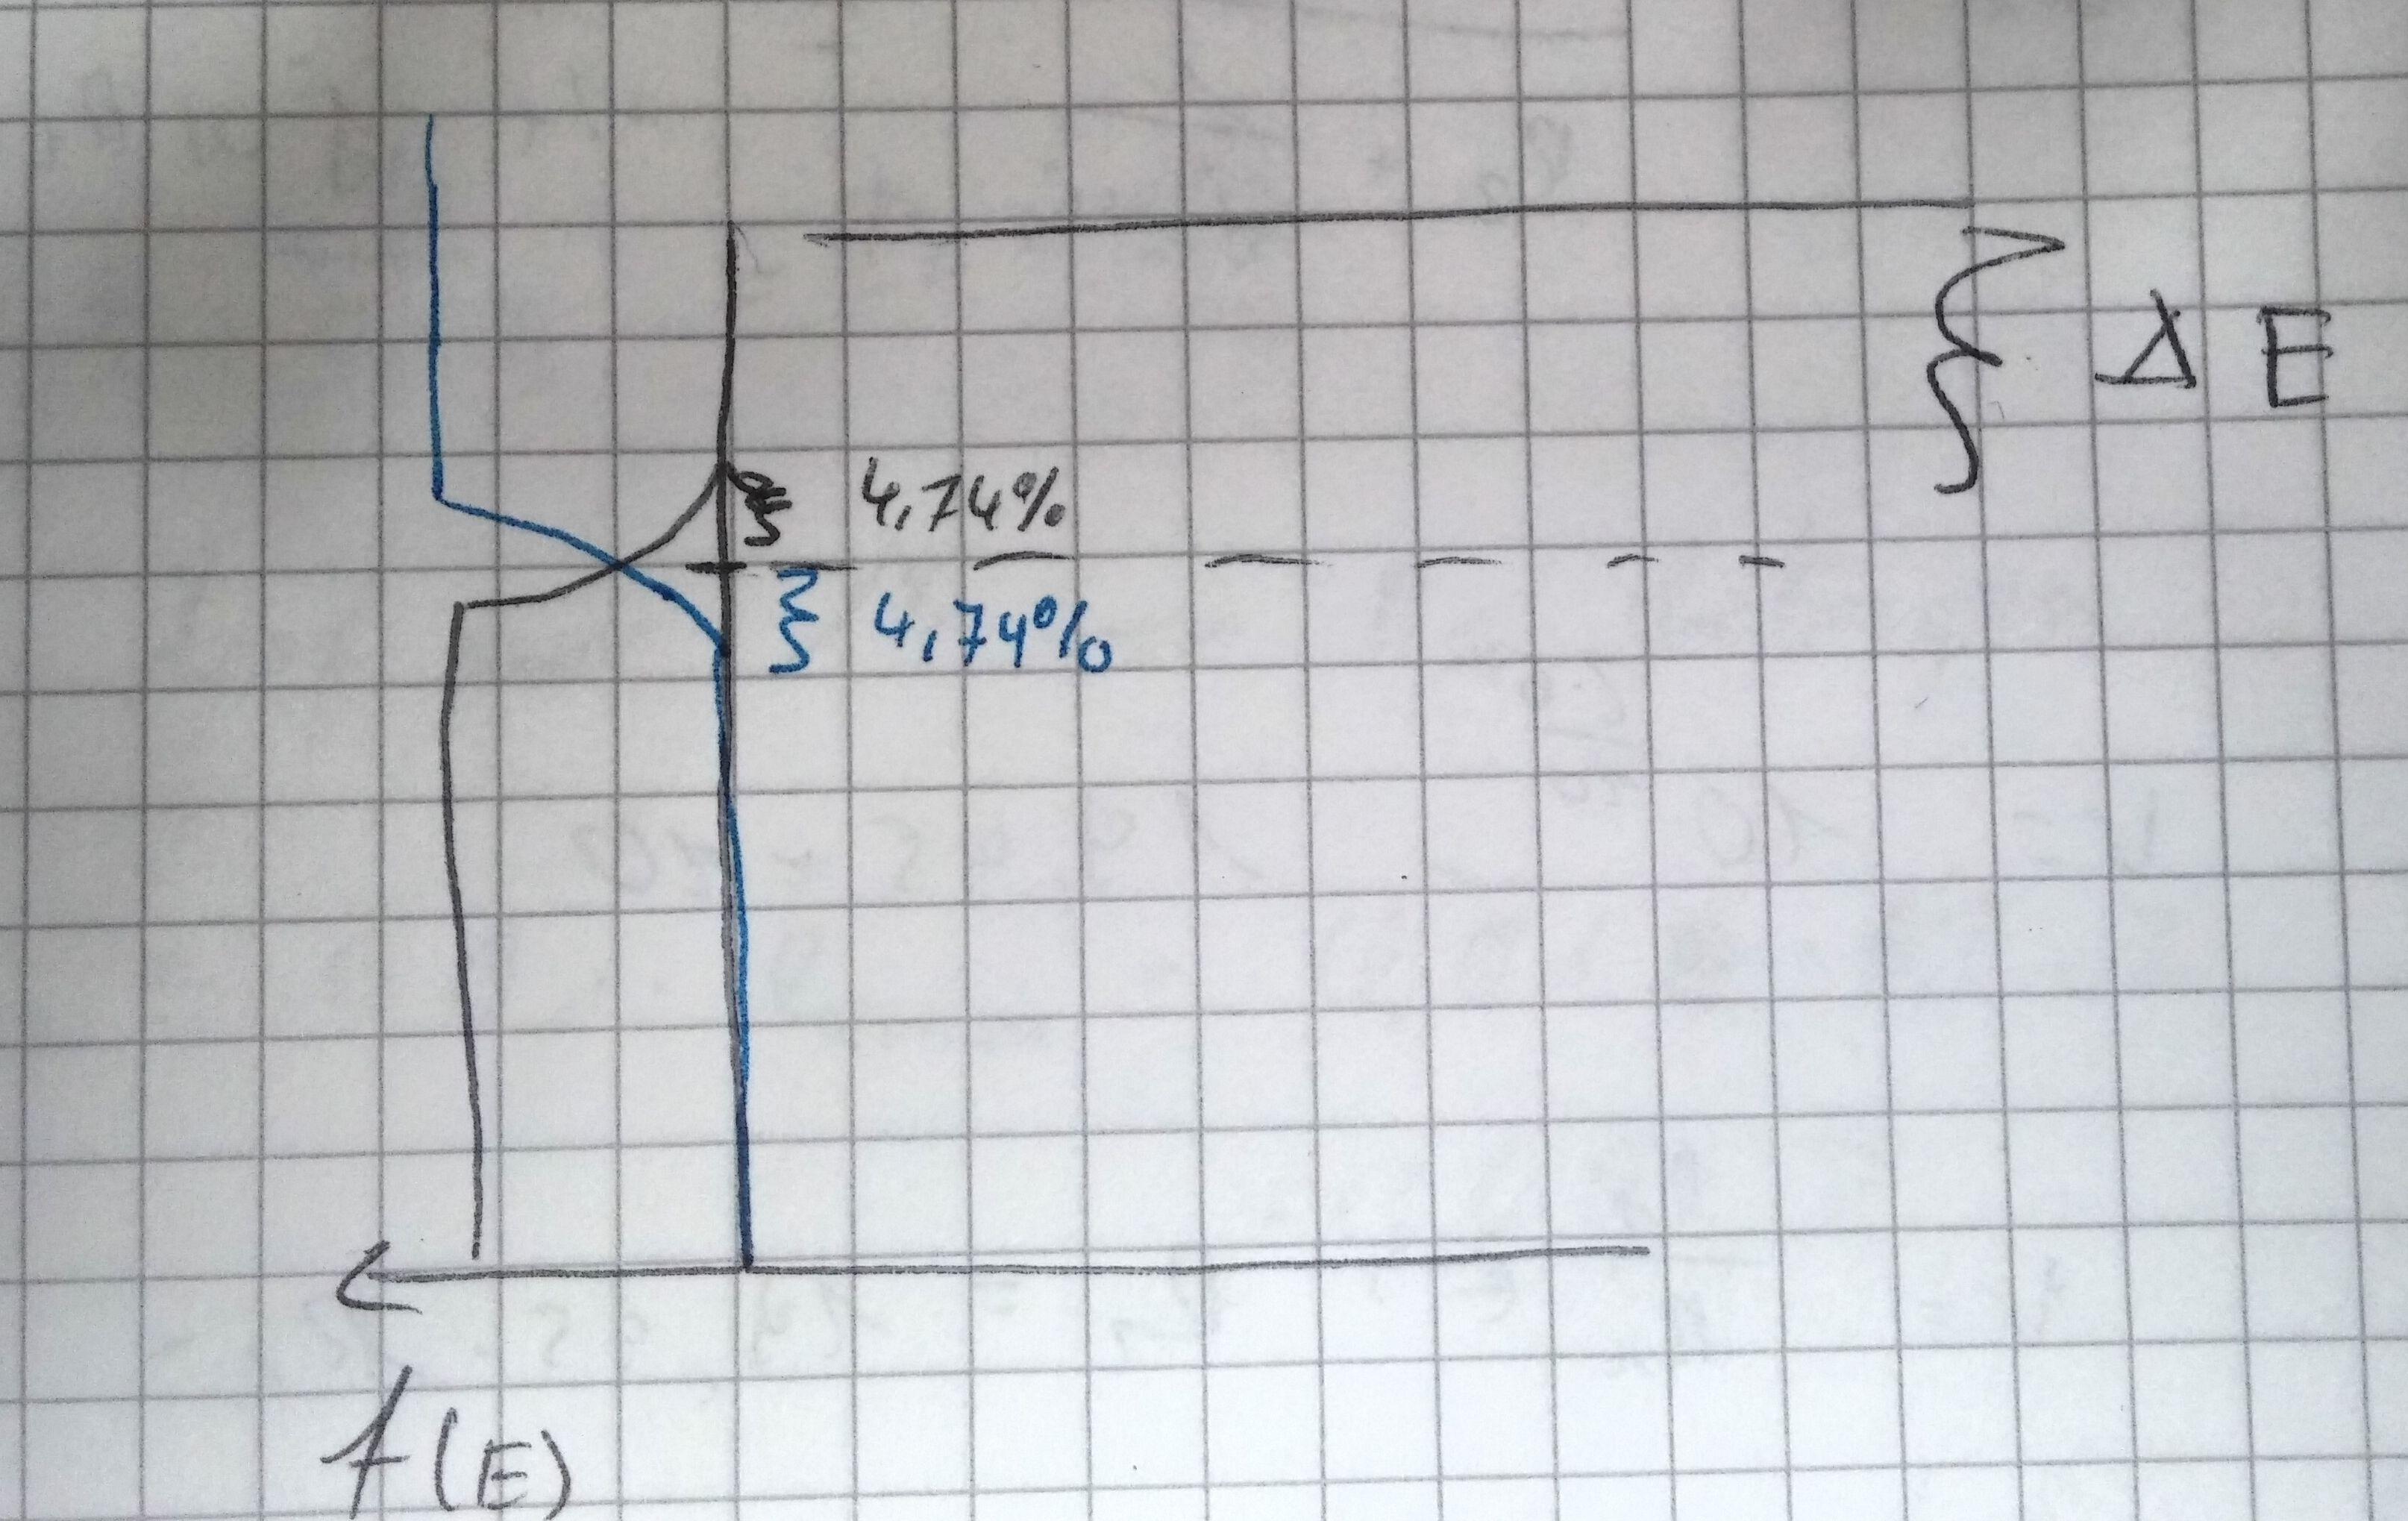
\includegraphics[scale=0.1]{A6_1.jpg}
\end{figure}


Das zeitliche verhalten sähe in einer Formel so aus:

\begin{align*}
P(t) &= P_E + (P_0 - P_E) \cdot e^{- \frac{t}{\tau}}
\intertext{$\tau$ ist in diesem Fall:}
\tau &= \frac{V_{rez}}{S_{eff}} = \frac{1}{1} = \unit[1]{s} 
\intertext{Damit gilt:}
P(t) &= P_E + (10^{-3} - P_E) \cdot e^{- \frac{t}{1}}
\end{align*}


\subsection*{b)}

Für den Enddruck gilt das Gleichgewicht zwischen Leckrate und Abpumprate:

\begin{align*}
P_a \cdot C_{Leck} &= P_E \cdot S_{Pumpe} 
\intertext{Unsere Leckrate ist dabei:}
C_{Leck} &= 117,6 \cdot A = 117,6 \cdot \frac{\left( 10^{-6} \right)^2 \cdot \pi}{4} = \unit[9,2 \cdot 10^{-8}]{l/s}
\intertext{Wir formen nach $P_E$ um:}
P_E &= \frac{P_A \cdot C_{Leck}}{S_{Pumpe}} = \frac{1000 \cdot 9,2 \cdot 10^{-8}}{1000} = \unit[9,2 \cdot 10^{-8}]{mbar}
\end{align*}


\subsection*{c)}

\begin{align*}
9,2 \cdot 10^{-8} \cdot 1000 &= \unit[9,2 \cdot 10^{-5}]{mbar \ l/s} \qquad \textcolor{red}{Warum????}
\intertext{Die anderen Leckraten ergeben sich darüber:}
C_{H_2} &= C_{N_2} \cdot \sqrt{\frac{28}{2}} = 9,2 \cdot 10^{-5} \cdot 3,2 = \unit[3,44 \cdot 10^{-4}]{mbar \ l/s} \\
C_{H_2} &= C_{N_2} \cdot \sqrt{\frac{28}{2}} = \unit[3,44 \cdot 10^{-4}]{mbar \ l/s} \\
C_{O_2} &= C_{N_2} \cdot \sqrt{\frac{28}{32}} = \unit[8,6 \cdot 10^{-5}]{mbar \ l/s} \\
C_{He} &= C_{N_2} \cdot \sqrt{\frac{28}{4}} = \unit[2,4 \cdot 10^{-4}]{mbar \ l/s}
\end{align*}


\subsection*{d)}

Wir nehmen vereinfacht an:

\begin{align*}
P &\sim P_0 \cdot e^{- \frac{t}{\tau}} \\
\Leftrightarrow - \frac{t}{\tau} &= \ln\left( \frac{P}{P_0} \right) \\
\Leftrightarrow t &= - \tau \cdot \ln\left( \frac{P}{P_0} \right) = 1 \cdot \ln\left( 10^{-3} \right) = \unit[6,9]{s}
\end{align*}



\section{Aufgabe 7}

Die mittlere freie Weglänge von $N_2$ können wir so bestimmen:

\begin{align*}
\Lambda_{N_2} &= \frac{1}{\pi \sqrt{2} d^2 n} = \frac{kT}{\pi \sqrt{2} d^2 P} = \unit[97]{\mu m}
\end{align*}

Bei TMG müssen wir zunächst das Volumen und darüber den Durchmesser errechnen:

\begin{align*}
\rho &= \frac{m}{V_0} = \frac{\frac{M}{L_A}}{V_0} \qquad V_0 = \text{Volumen des Moleküls} \qquad L_A = \text{Avogadrozahl} \\
V_0 &= \frac{M}{L_A \cdot rho} = \frac{114,82}{6,022 \cdot 10^{22} \cdot 1,159} = \unit[1,66 \cdot 10^{-22}]{ml} = \unit[1,66 \cdot 10^{-28}]{m^3} \\
\intertext{Nun können wir den Durchmesser berechnen:}
V_0 &= \frac{4}{3} \pi r^3 \Leftrightarrow r_0 = \unit[3,4 \cdot 10^{-10}]{m} \Rightarrow d = \unit[6,8 \cdot 10^{-10}]{m}
\intertext{Wir setzen in die Formel ein, die wir auch schon beim ersten Stoff verwendet haben:}
\Lambda_{TMG} &= \frac{3,1 \cdot 10^{-24} \cdot 300}{100 \cdot \left( 6,8 \cdot 10^{-10} \right)^2} = \unit[20]{\mu m}
\intertext{Bei $AsT_3$ können wir auch einfach einsetzen:}
\Lambda_{AsT_3} &= \frac{3,1 \cdot 10^{-24} \cdot 300}{100 \cdot \left( 2 \cdot 185 \cdot 10^{-12} \right)^2} = \unit[68]{\mu m}
\end{align*}


\section{Aufgabe 8}


\subsection*{a)}

Wir berechnen zunächst $\lambda$, das wir dann in die Knudsengleichung einsetzen:

\begin{align*}
\lambda &= \frac{\unit[68]{\mu m}}{\unit[2]{mbar}} = \unit[34]{\mu m /mbar} 
\intertext{Nun können wir einsetzen:}
K &= \frac{\lambda}{D} = \frac{34 \cdot 10^{-6}}{35 \cdot 10^{-3}} \approx 10^{-3} < 0,2
\end{align*}

Damit liegt eine laminare Strömung vor. Die nachfolgenden Aufgabenteile folgen dem selben Prinzip.


\subsection*{b)}

\begin{align*}
\lambda &= \frac{\unit[115]{\mu m}}{\unit[2]{mbar}} = \unit[57,5]{\mu m /mbar} 
\intertext{Nun können wir einsetzen:}
K &= \frac{\lambda}{D} = \frac{57,5 \cdot 10^{-6}}{6 \cdot 10^{-3}} = 9,5 \cdot 10^{-2} < 0,2
\end{align*}

Das noch grade so eine laminare Strömung.


\subsection*{c)}

\begin{align*}
\lambda &= \frac{\unit[68]{\mu m}}{\unit[10^{-6}]{mbar}} = \unit[68]{m /mbar} 
\intertext{Nun können wir einsetzen:}
K &= \frac{\lambda}{D} = \frac{68}{0,05} = 68 \cdot 10^{-3} > 0,5
\end{align*}

Das ist eine molekulare Strömung.


\subsection*{d)}

\begin{align*}
\lambda &= \frac{\unit[68]{\mu m}}{\unit[10^{-3}]{mbar}} = \unit[68 \cdot 10^{-3}]{m /mbar} 
\intertext{Nun können wir einsetzen:}
K &= \frac{\lambda}{D} = \frac{68 \cdot 10^{-3}}{35 \cdot 10^{-3}} = 1,9 > 0,5
\end{align*}

Das ist eine molekulare Strömung.

\newpage


\section{Aufgabe 9}


Diese Aufgabe geht im Prinzip wie die Aufgabe 8, nur das es jetzt um den Durchmesser geht:

\begin{align*}
\lambda &= \frac{\unit[68]{\mu m}}{\unit[10^{-3}]{mbar}} = \unit[68 \cdot 10^{-3}]{m /mbar} \\
K < \frac{\lambda}{D} &\Leftrightarrow D < \frac{\lambda}{K} = \frac{68 \cdot 10^{-3}}{0,5} = \unit[0,169]{m}
\end{align*}


\section{Aufgabe 10}

\subsection*{a)}

Wir bestimmen zunächst wiederum $\lambda$:

\begin{align*}
\lambda &= \frac{\unit[68]{\mu m}}{1000]{mbar}} = \unit[68 \cdot 10^{-9}]{m /mbar} 
\intertext{Wir gehen davon aus, das wir mit $<v> = \unit[470]{m/s}$ rechnen können:}
D &= \frac{68 \cdot 10^{-9} \cdot 470}{3} = \unit[1,06 \cdot 10^{-5}]{m^2/s}
\intertext{Für die Diffusionslänge setzen wir nun an:}
L \sim 3 \cdot \sqrt{D \cdot t} = 3 \cdot \sqrt{1,06 \cdot 10^{-5} \cdot 5 \cdot 60} = \unit[0,169]{m}
\end{align*}


\subsection*{b)}

\begin{align*}
v_D &= \frac{L}{t} = \frac{0,169}{300} = \unit[4,6 \cdot 10^{-4}]{m/s}
\end{align*}
























\end{document}